\chapter{\heiti 软件使用}
\section{\heiti 打开控制软件}
进入我司为用户提供的Integration的文件夹,双击运行“ASG.py”文件,即可打开方波序列编辑软件。软件主界面(Pulse界面)如图4.1所示。
\begin{figure}[ht]
\centering
%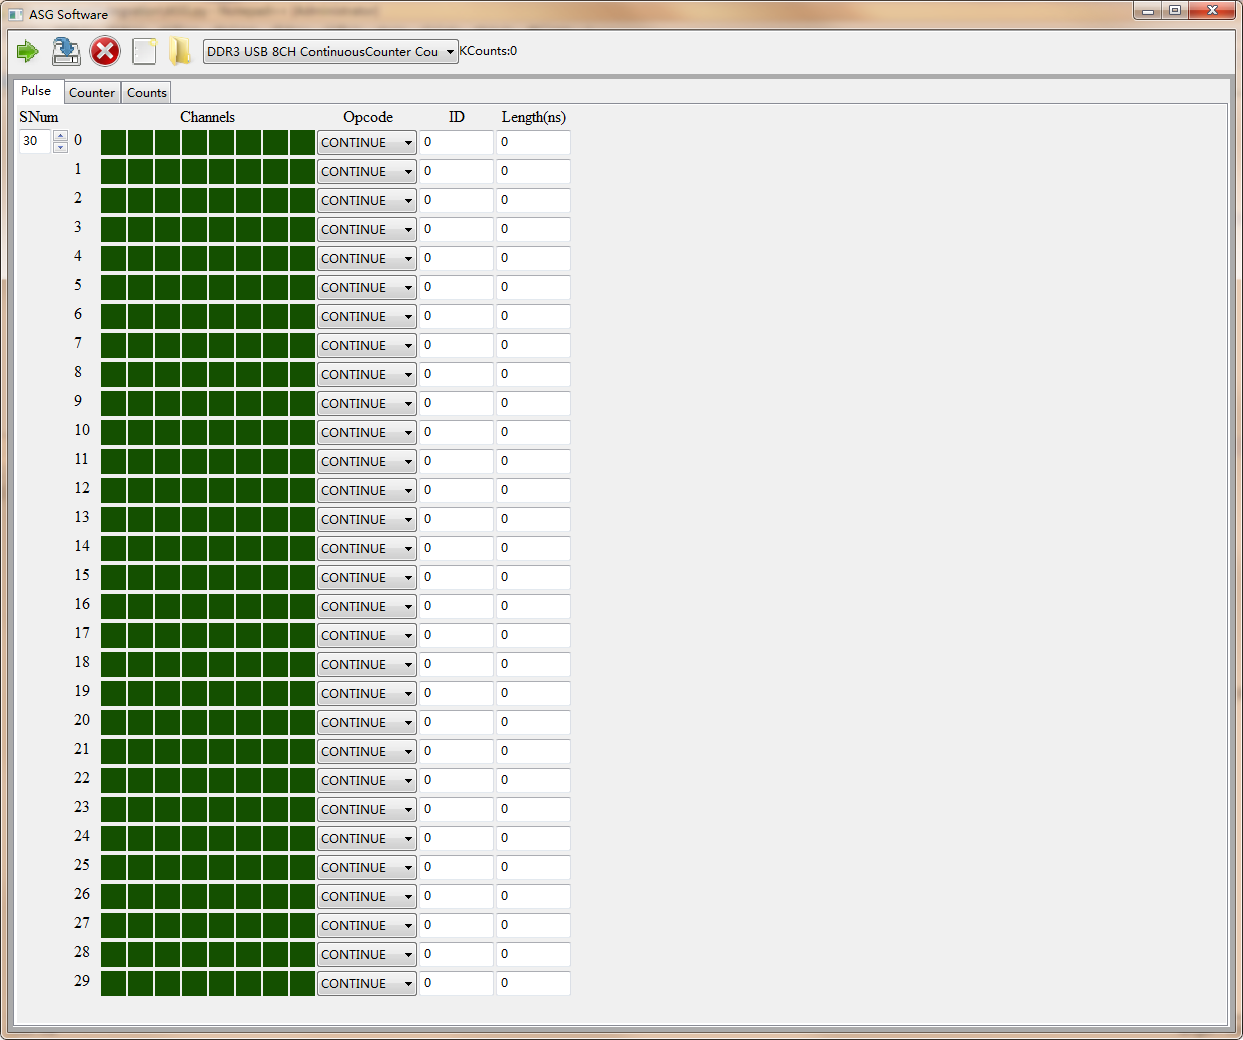
\includegraphics[width=11cm,height=9cm]{fig4_1}
%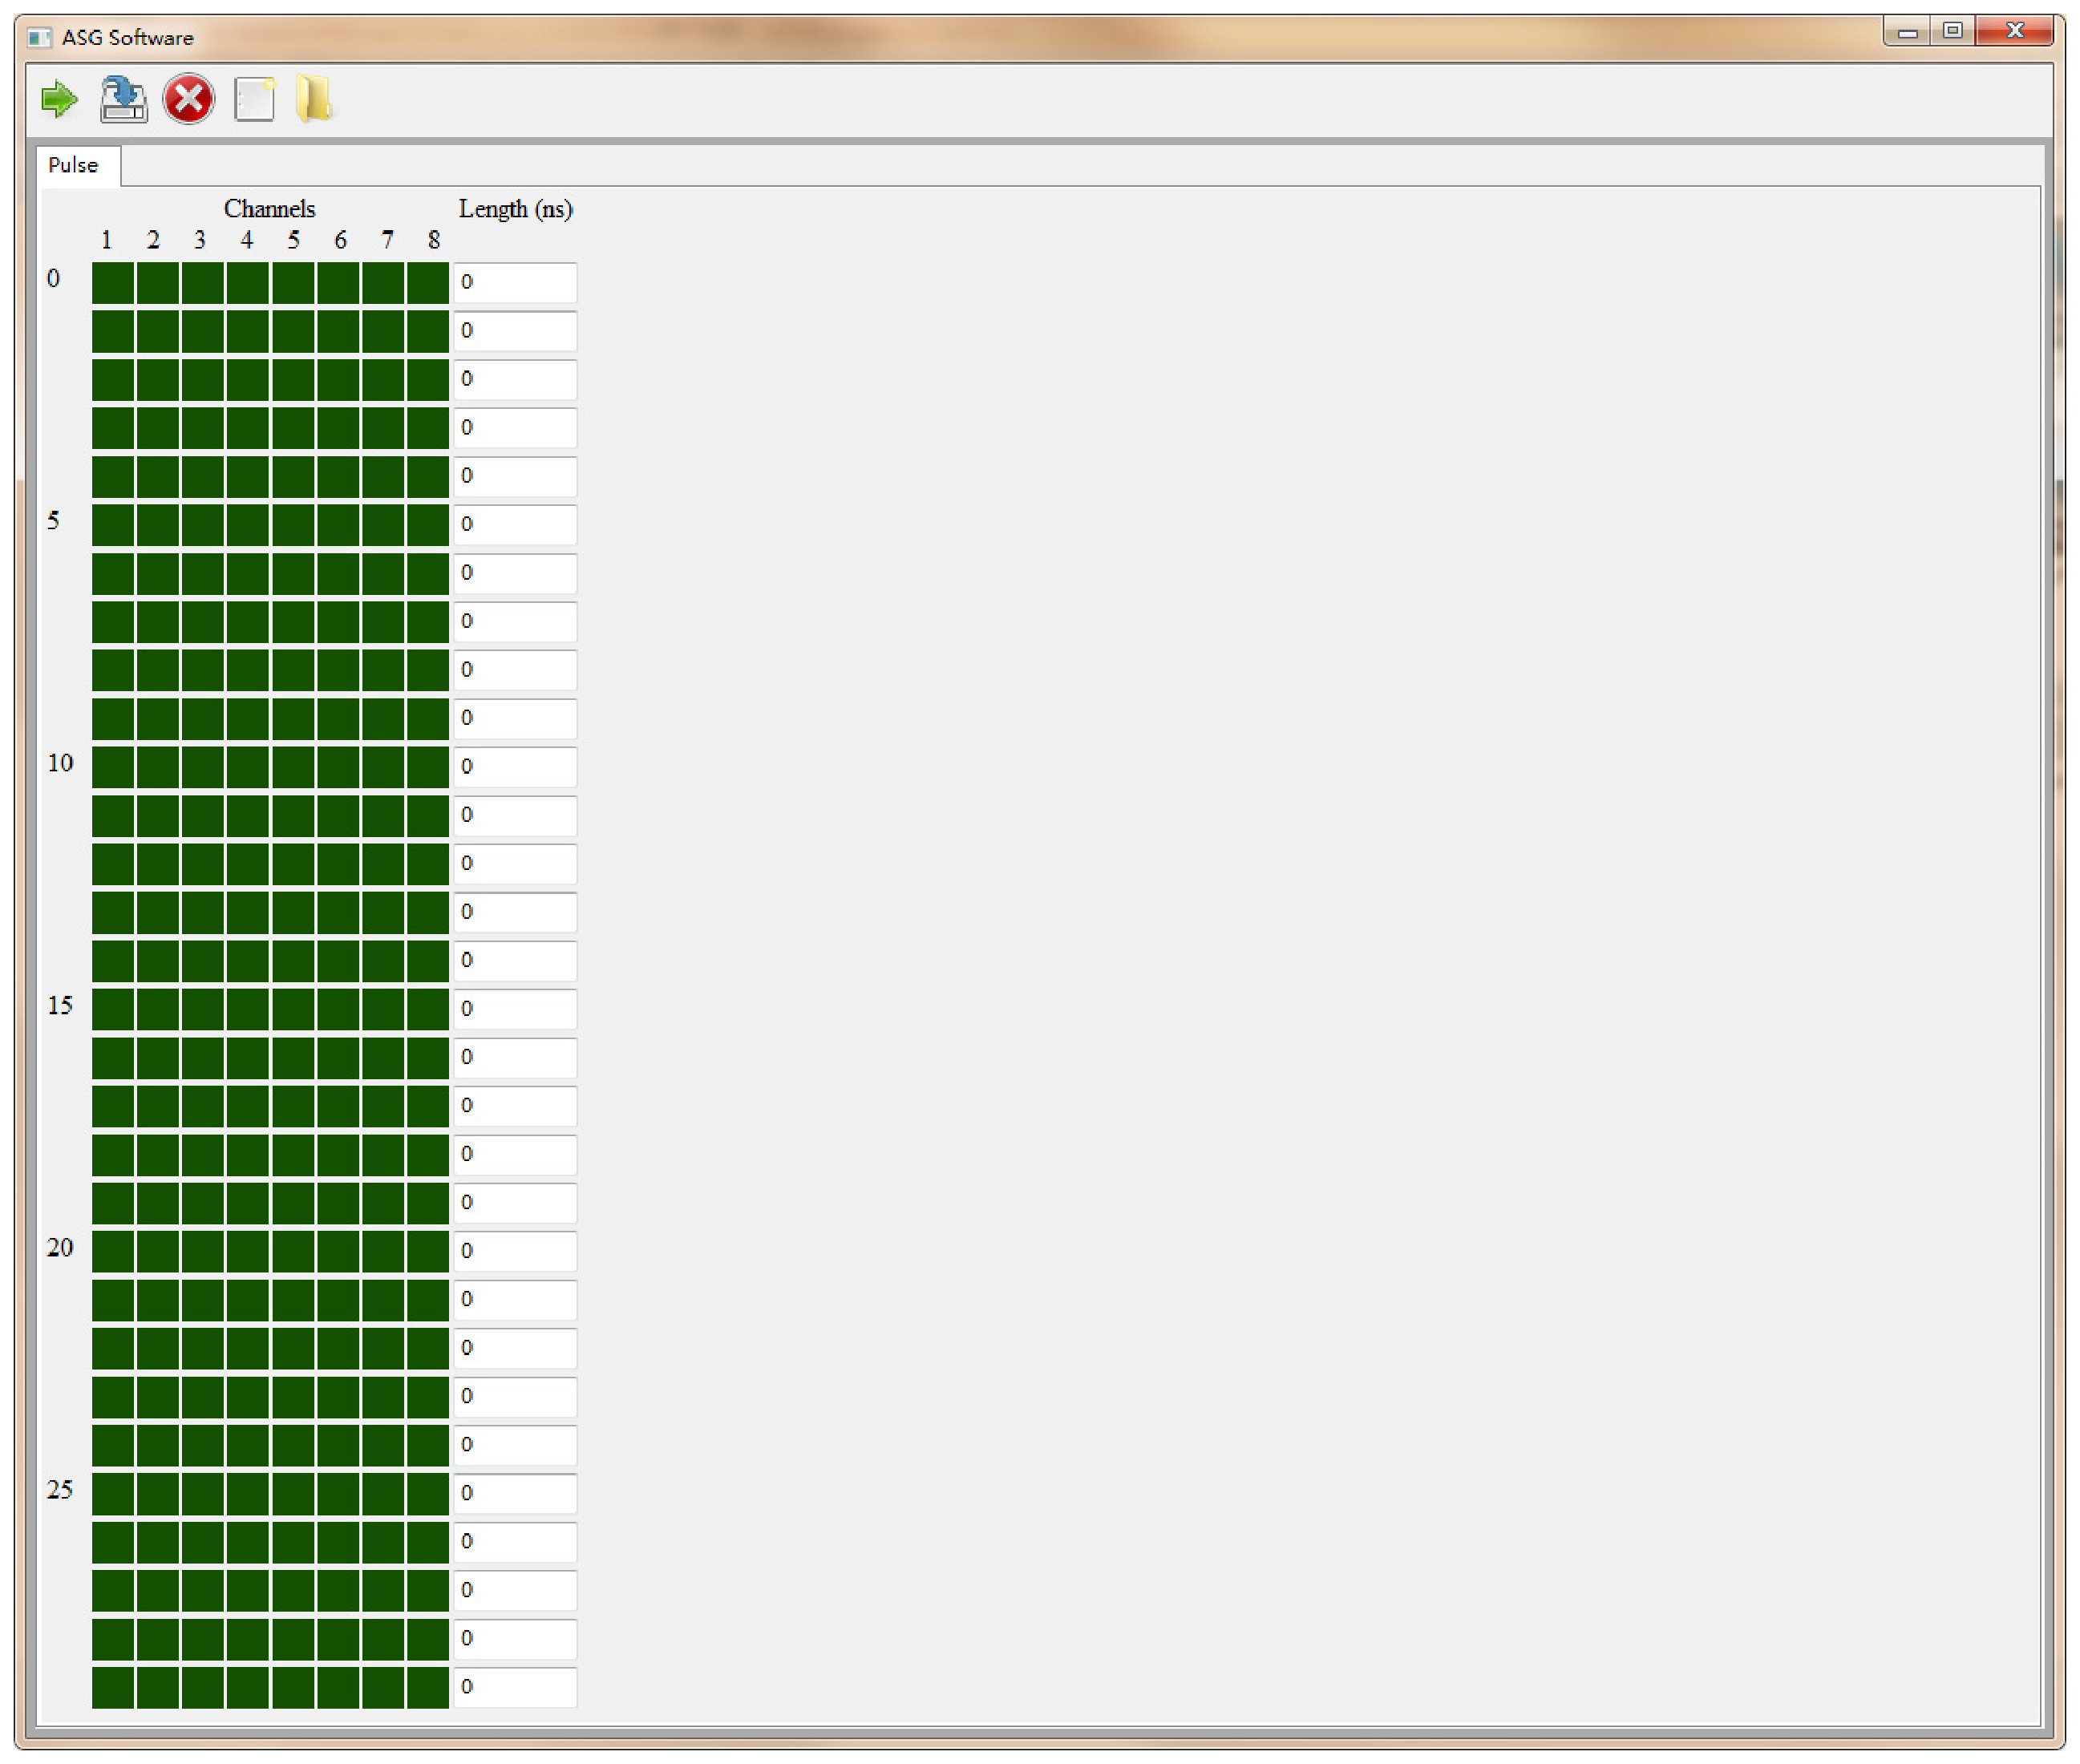
\includegraphics[width=12cm,height=9cm]{fig4_1_xyj}
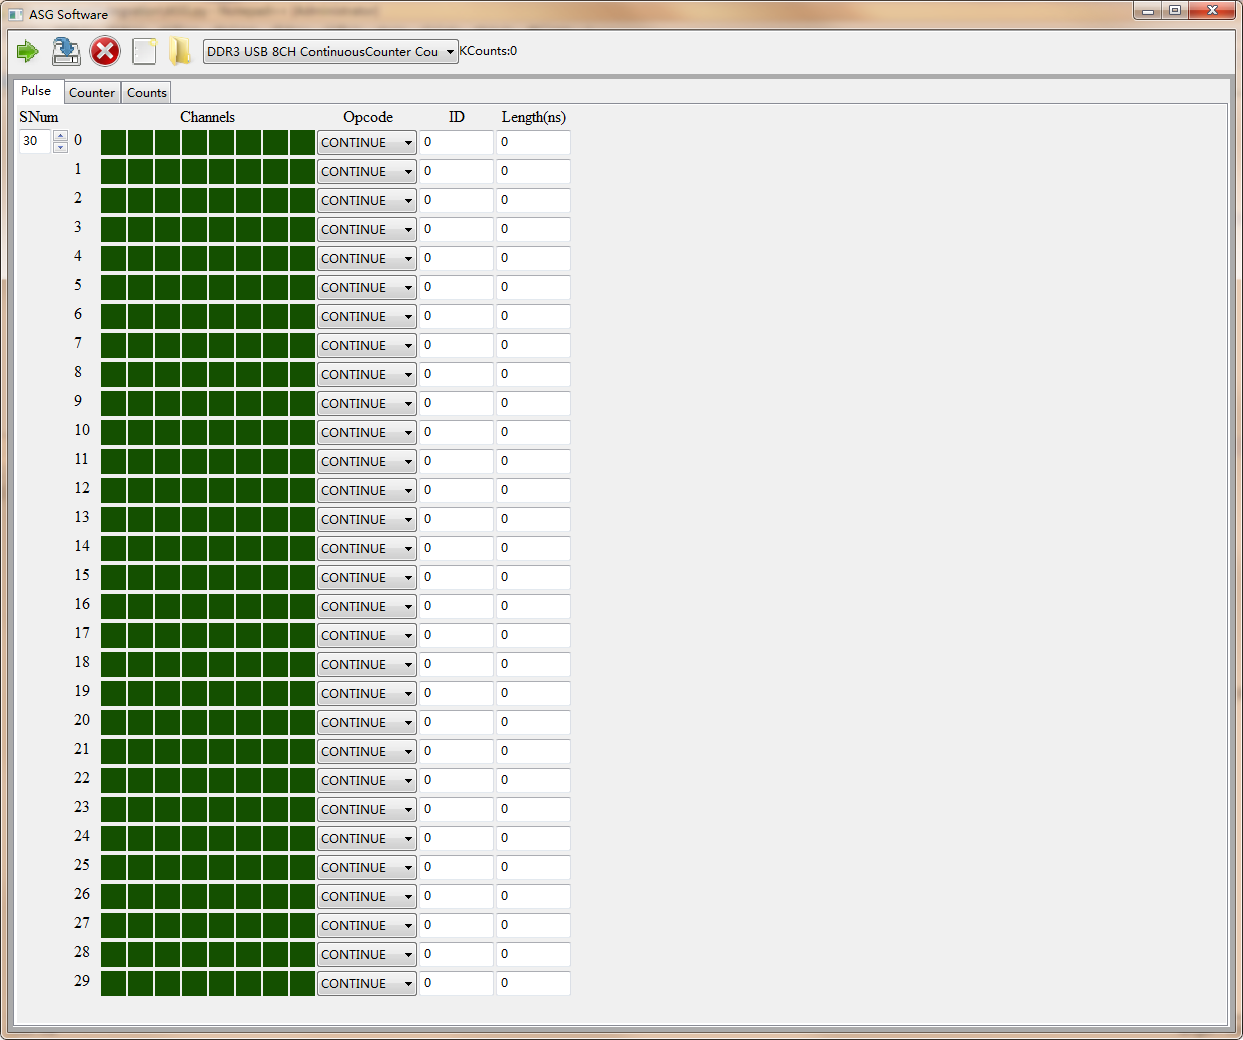
\includegraphics[height=9cm]{fig4_1}
\caption{软件主界面}
\end{figure}

在软件主界面工具栏中,从左往右5个按钮依次为:“开始播放按钮”、“下载方波数据按钮”、“停止播放按钮”、“存储当前方波序列按钮”、“载入存储方波序列按钮”。界面中间的每行8个绿色方框,从左往右依次代表OUT 1 至OUT 8 的8 个方波输出通道在一段时间内的输出状态(时间长度由右侧的“Length” 文本框内输入的数值决定,单位为纳秒)。当绿色被点亮时,该通道在此段时间内的输出为高电平;若绿色未被点亮,则该通道在此段时间内的输出为低电平。

\section{\heiti 定义任意方波序列举例}
用户可根据每行绿色方框的不同状态及“Length”的长度来定义任意的方波序列。如图4.2,左侧“CH - 1”至“CH - 4”代表4个方波输出通道,若用户想要生成如图4.2所示的方波序列,可如图4.3在软件界面中定义该方波序列。

\newpage
\vspace{0.6cm}
\begin{figure}[H]
\centering
%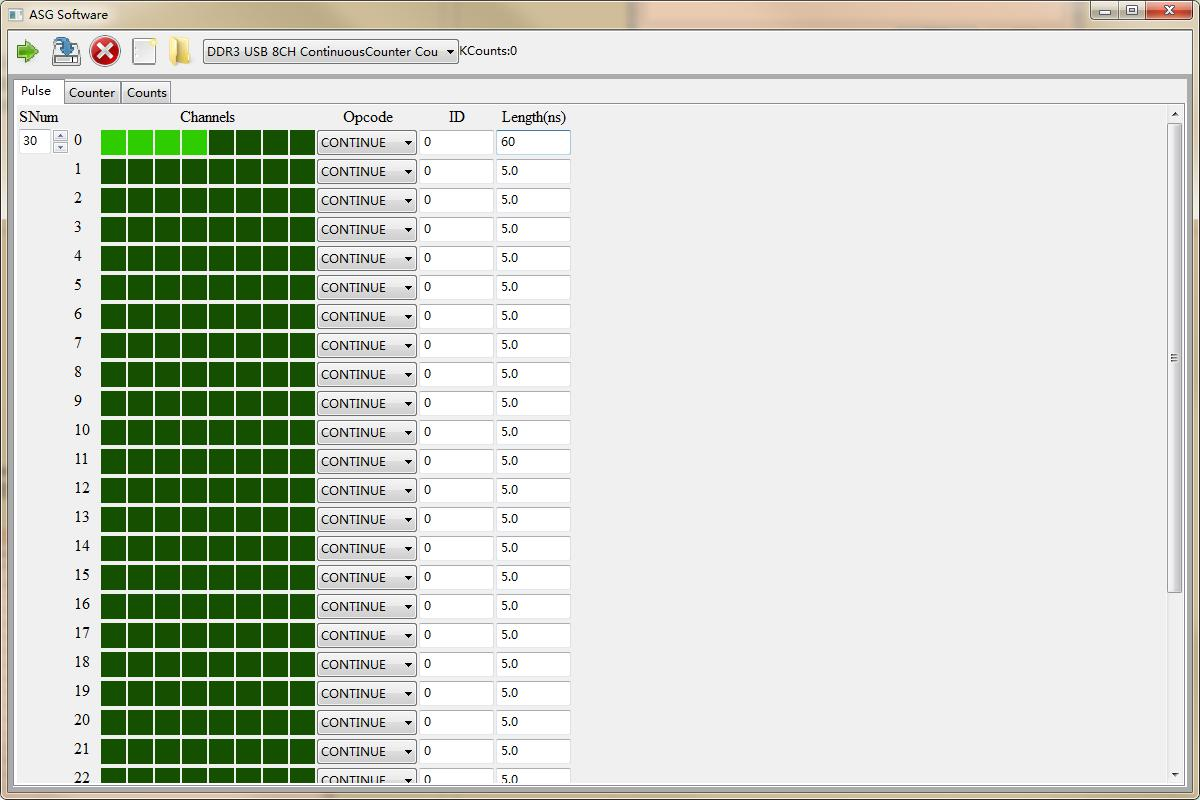
\includegraphics[width=11cm,height=9cm]{fig4_2}
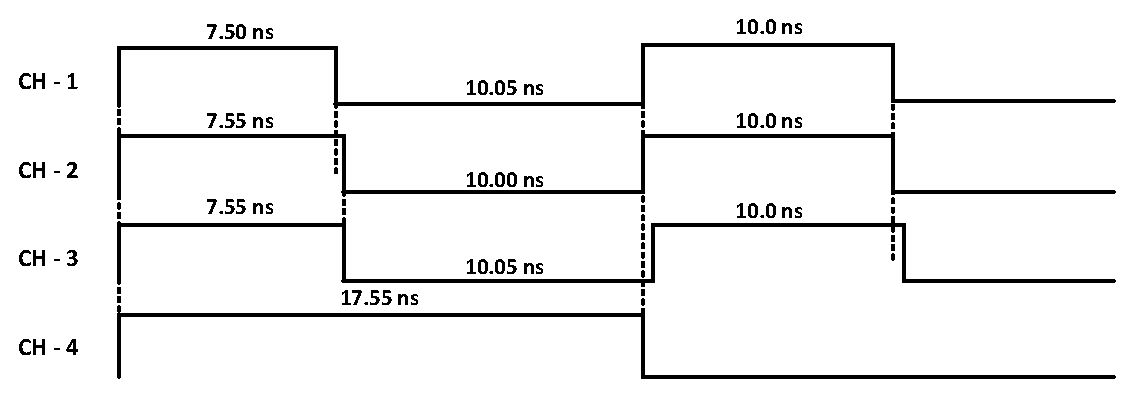
\includegraphics[height=5cm,width=14cm]{fig4_2_shixutu}
\caption{自定义方波序列时序图}
\end{figure}

\vspace{1cm}
\begin{figure}[H]
\centering
%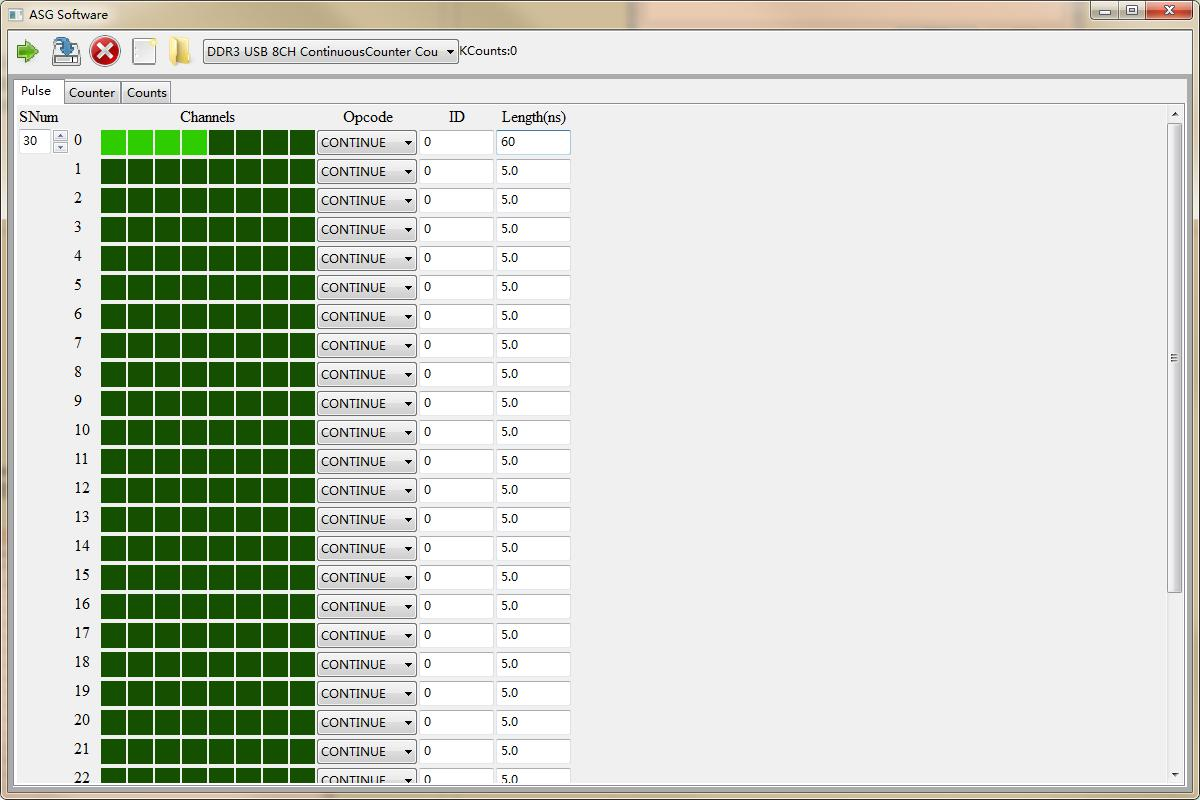
\includegraphics[width=11cm,height=9cm]{fig4_2}
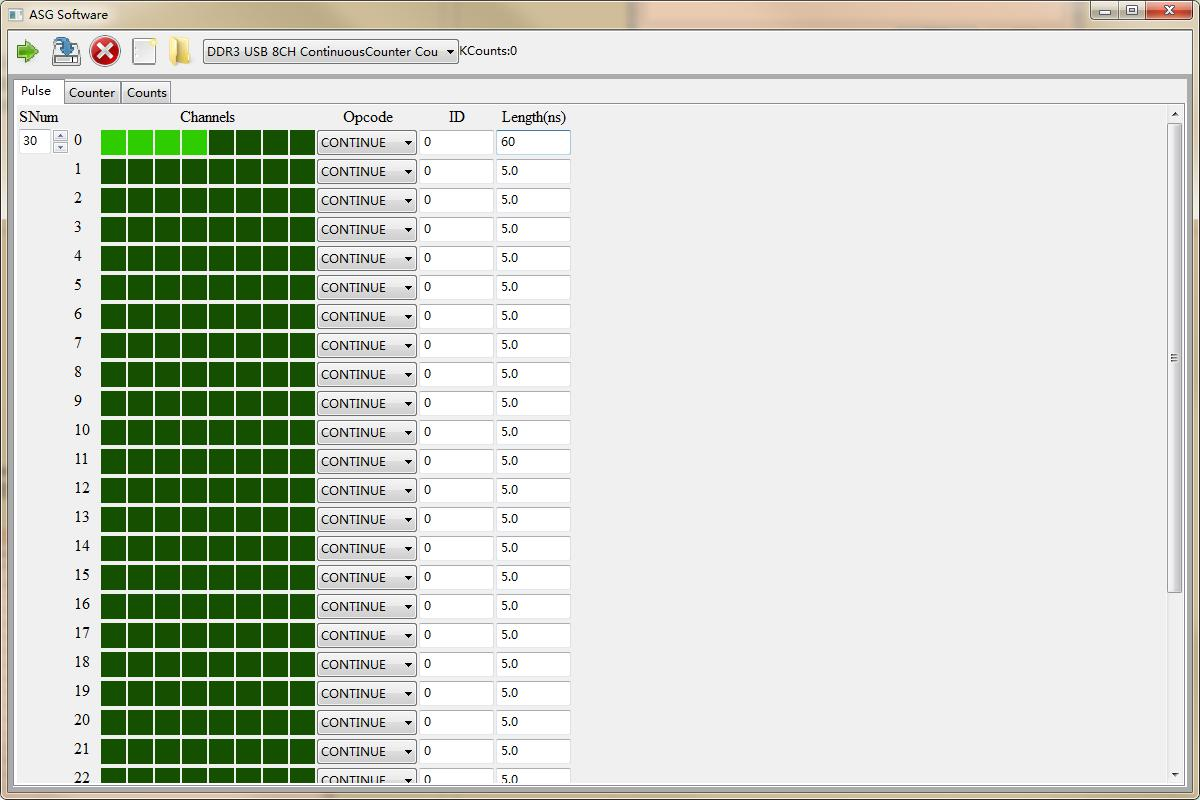
\includegraphics[height=9cm]{fig4_2}
\caption{使用软件定义方波序列}
\end{figure}
\vspace{0.6cm}
如图4.3使用方波编辑软件定义图4.2中的方波序列,这里只使用了4个方波输出通道,若用户需要同时使用更多的方波输出通道,可用同样的方法在其他通道定义任意方波序列。

\newpage
\section{\heiti 开始播放方波序列}
用户点击“Download”按钮
\includegraphics[height=0.7cm]{download},可将自定义的方波序列数据下载到硬件中。点击“Start”按钮
\includegraphics[height=0.7cm]{start},可使仪器各输出通道开始播放用户自定义的方波序列,在点击“Start” 按钮之前必须先将方波序列数据下载到硬件中。将输出通道用同轴线连接至示波器上可以看到仪器输出的方波波形。如用户定义图4.2所示方波序列,在示波器上可以看到如图4.4 所示的方波序列。

\vspace{2cm}

\begin{figure}[htbp]
\centering
%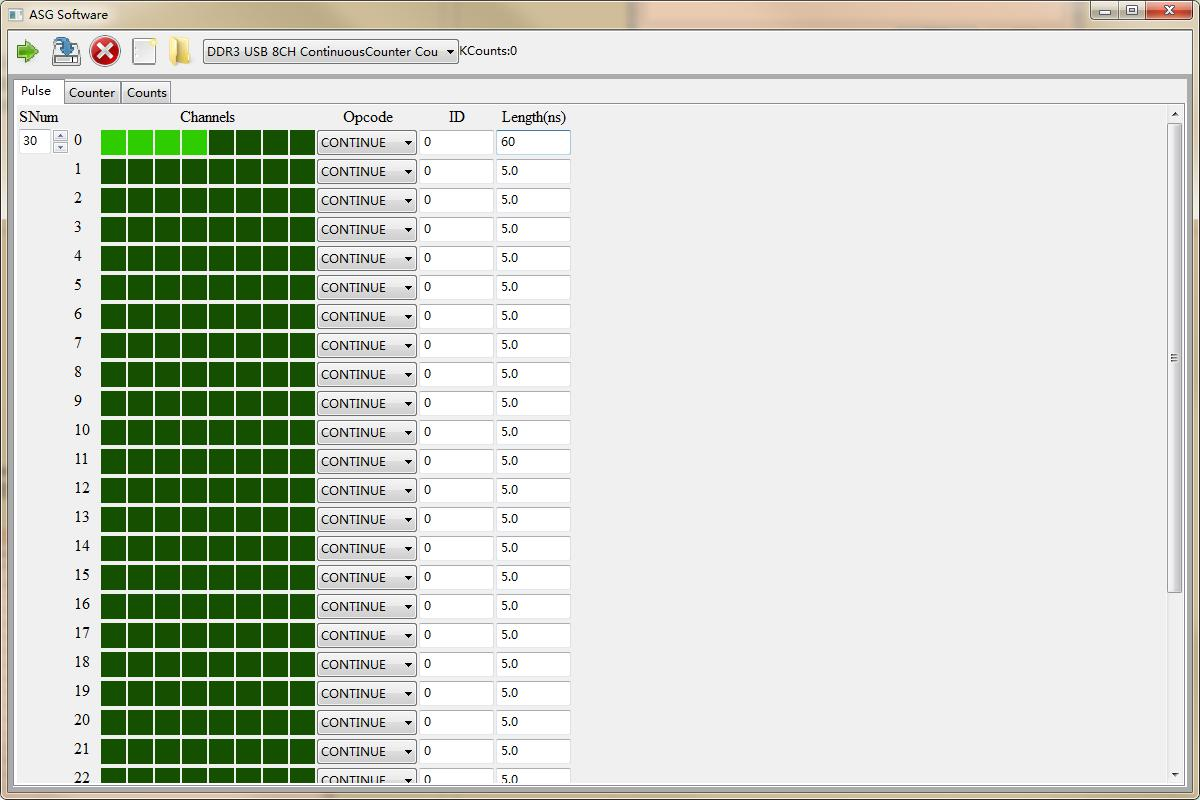
\includegraphics[width=11cm,height=9cm]{fig4_2}
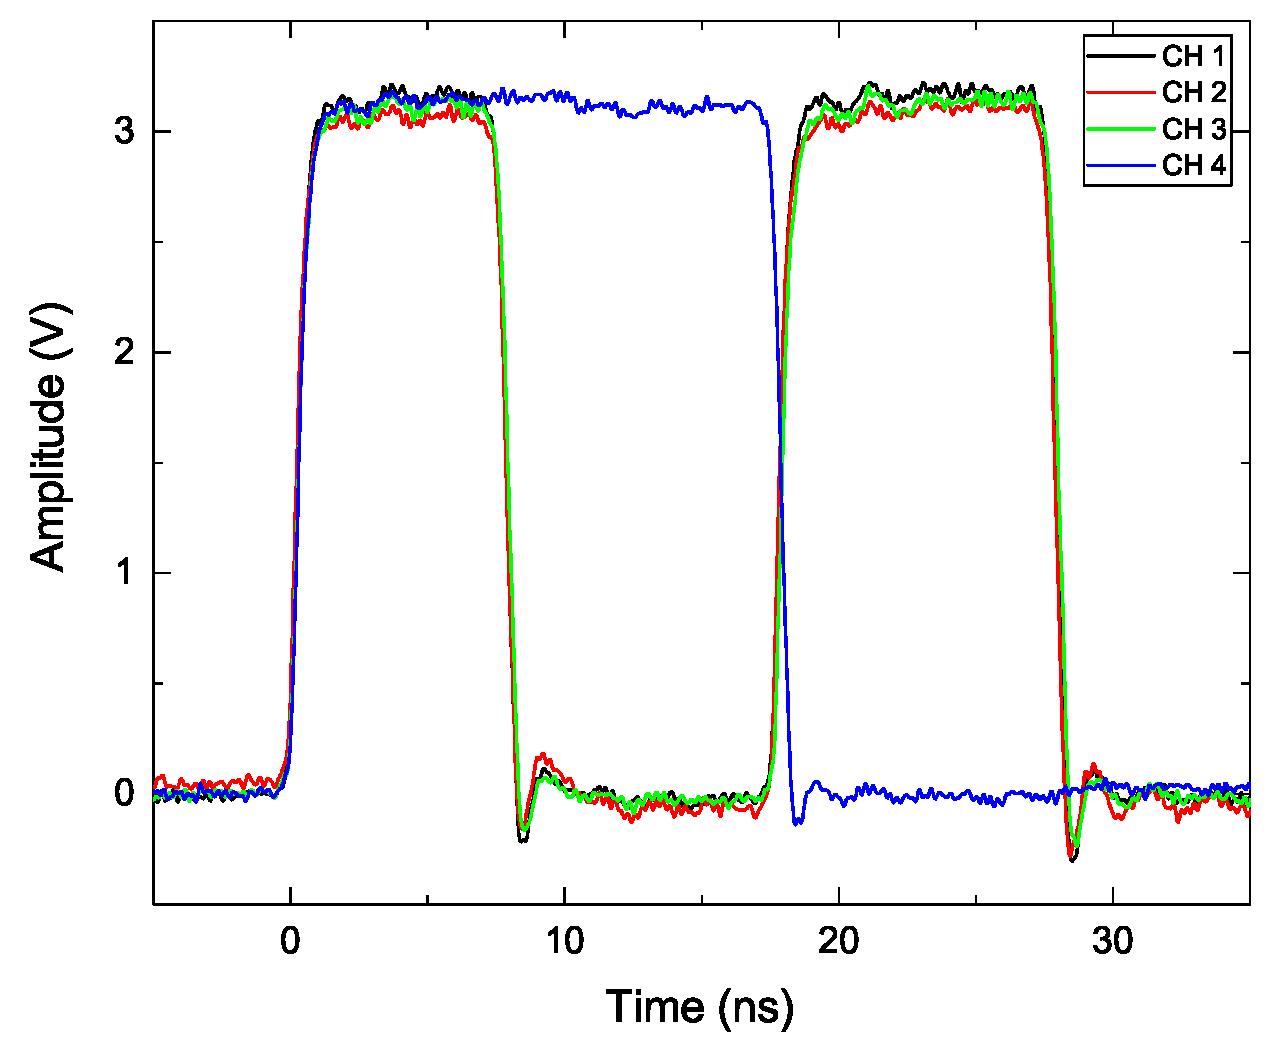
\includegraphics[height=9cm]{yangheng_shiboqi}
\caption{产品输出方波序列图}
\end{figure}


\section{\heiti 停止播放方波序列}
当仪器正在播放方波序列时,可以通过点击“Stop”按钮
\includegraphics[height=0.7cm]{stop}使仪器停止播放方波序列。


\newpage
\section{\heiti 定义方波序列注意事项}

\vspace{0.4cm}
\noindent \textbf{(1)}. 每个通道的方波序列中单个方波脉冲的高低电平时间必须在7.5 ns至2.6 s以内。如图4.5,当用户定义的方波序列中单个脉冲宽度小于7.5 ns 时,软件会弹出提示对话框让用户检查自定义的方波序列是否符合要求。

\vspace{0.2cm}
\begin{figure}[H]
\centering
%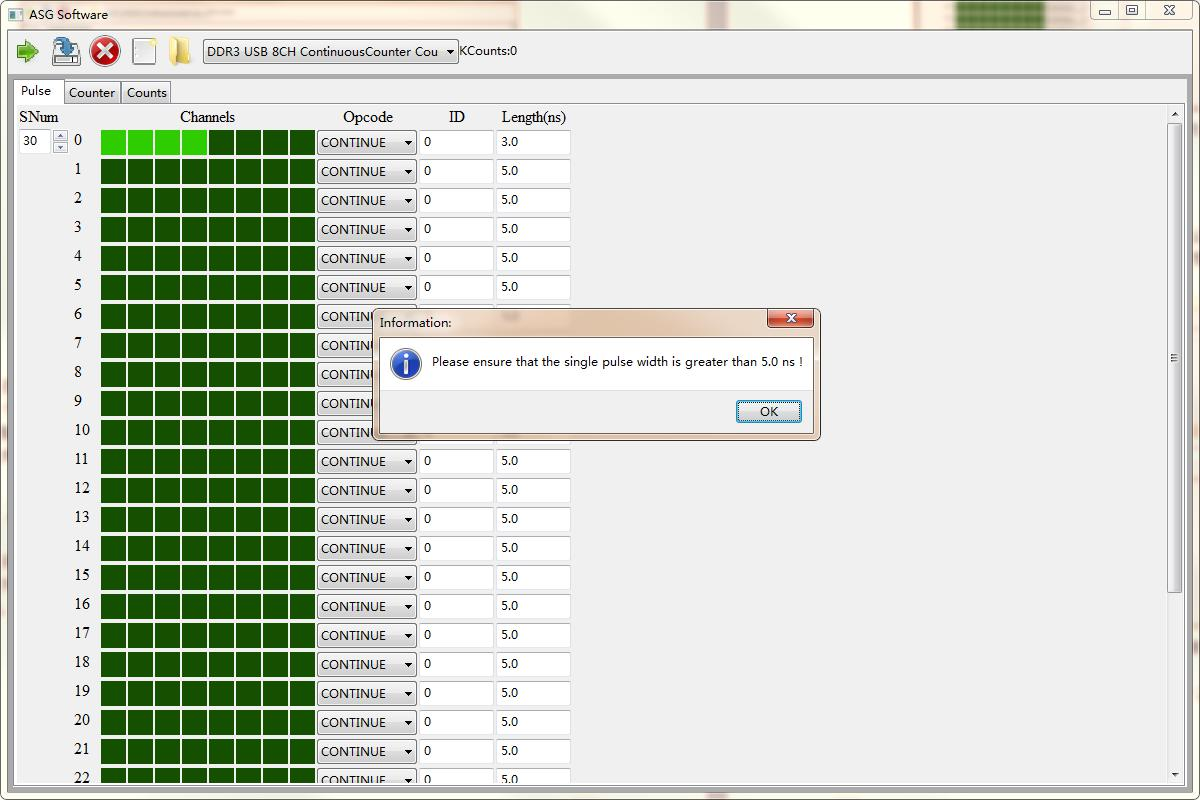
\includegraphics[width=11cm,height=9cm]{fig4_3}
%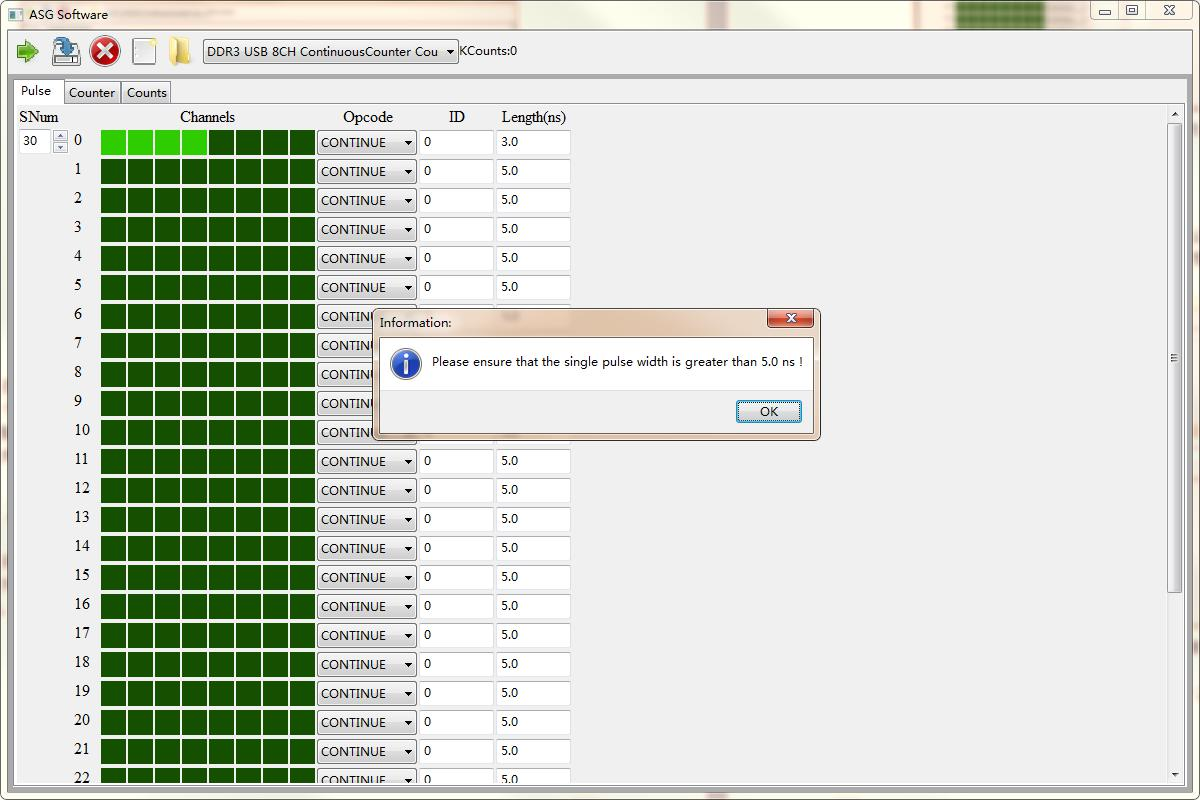
\includegraphics[height=9cm]{fig4_3}
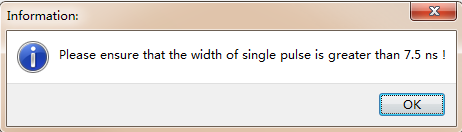
\includegraphics[height=3cm]{fig4_5_yh}
\caption{定义方波宽度小于7.5 ns提示}
\end{figure}

%\newpage
\vspace{0.4cm}
\noindent \textbf{(2)}.  如图4.6,当用户定义的方波序列中单个脉冲宽度大于2.6 s时,软件会弹出提示对话框。

\vspace{0.2cm}
\begin{figure}[ht]
\centering
%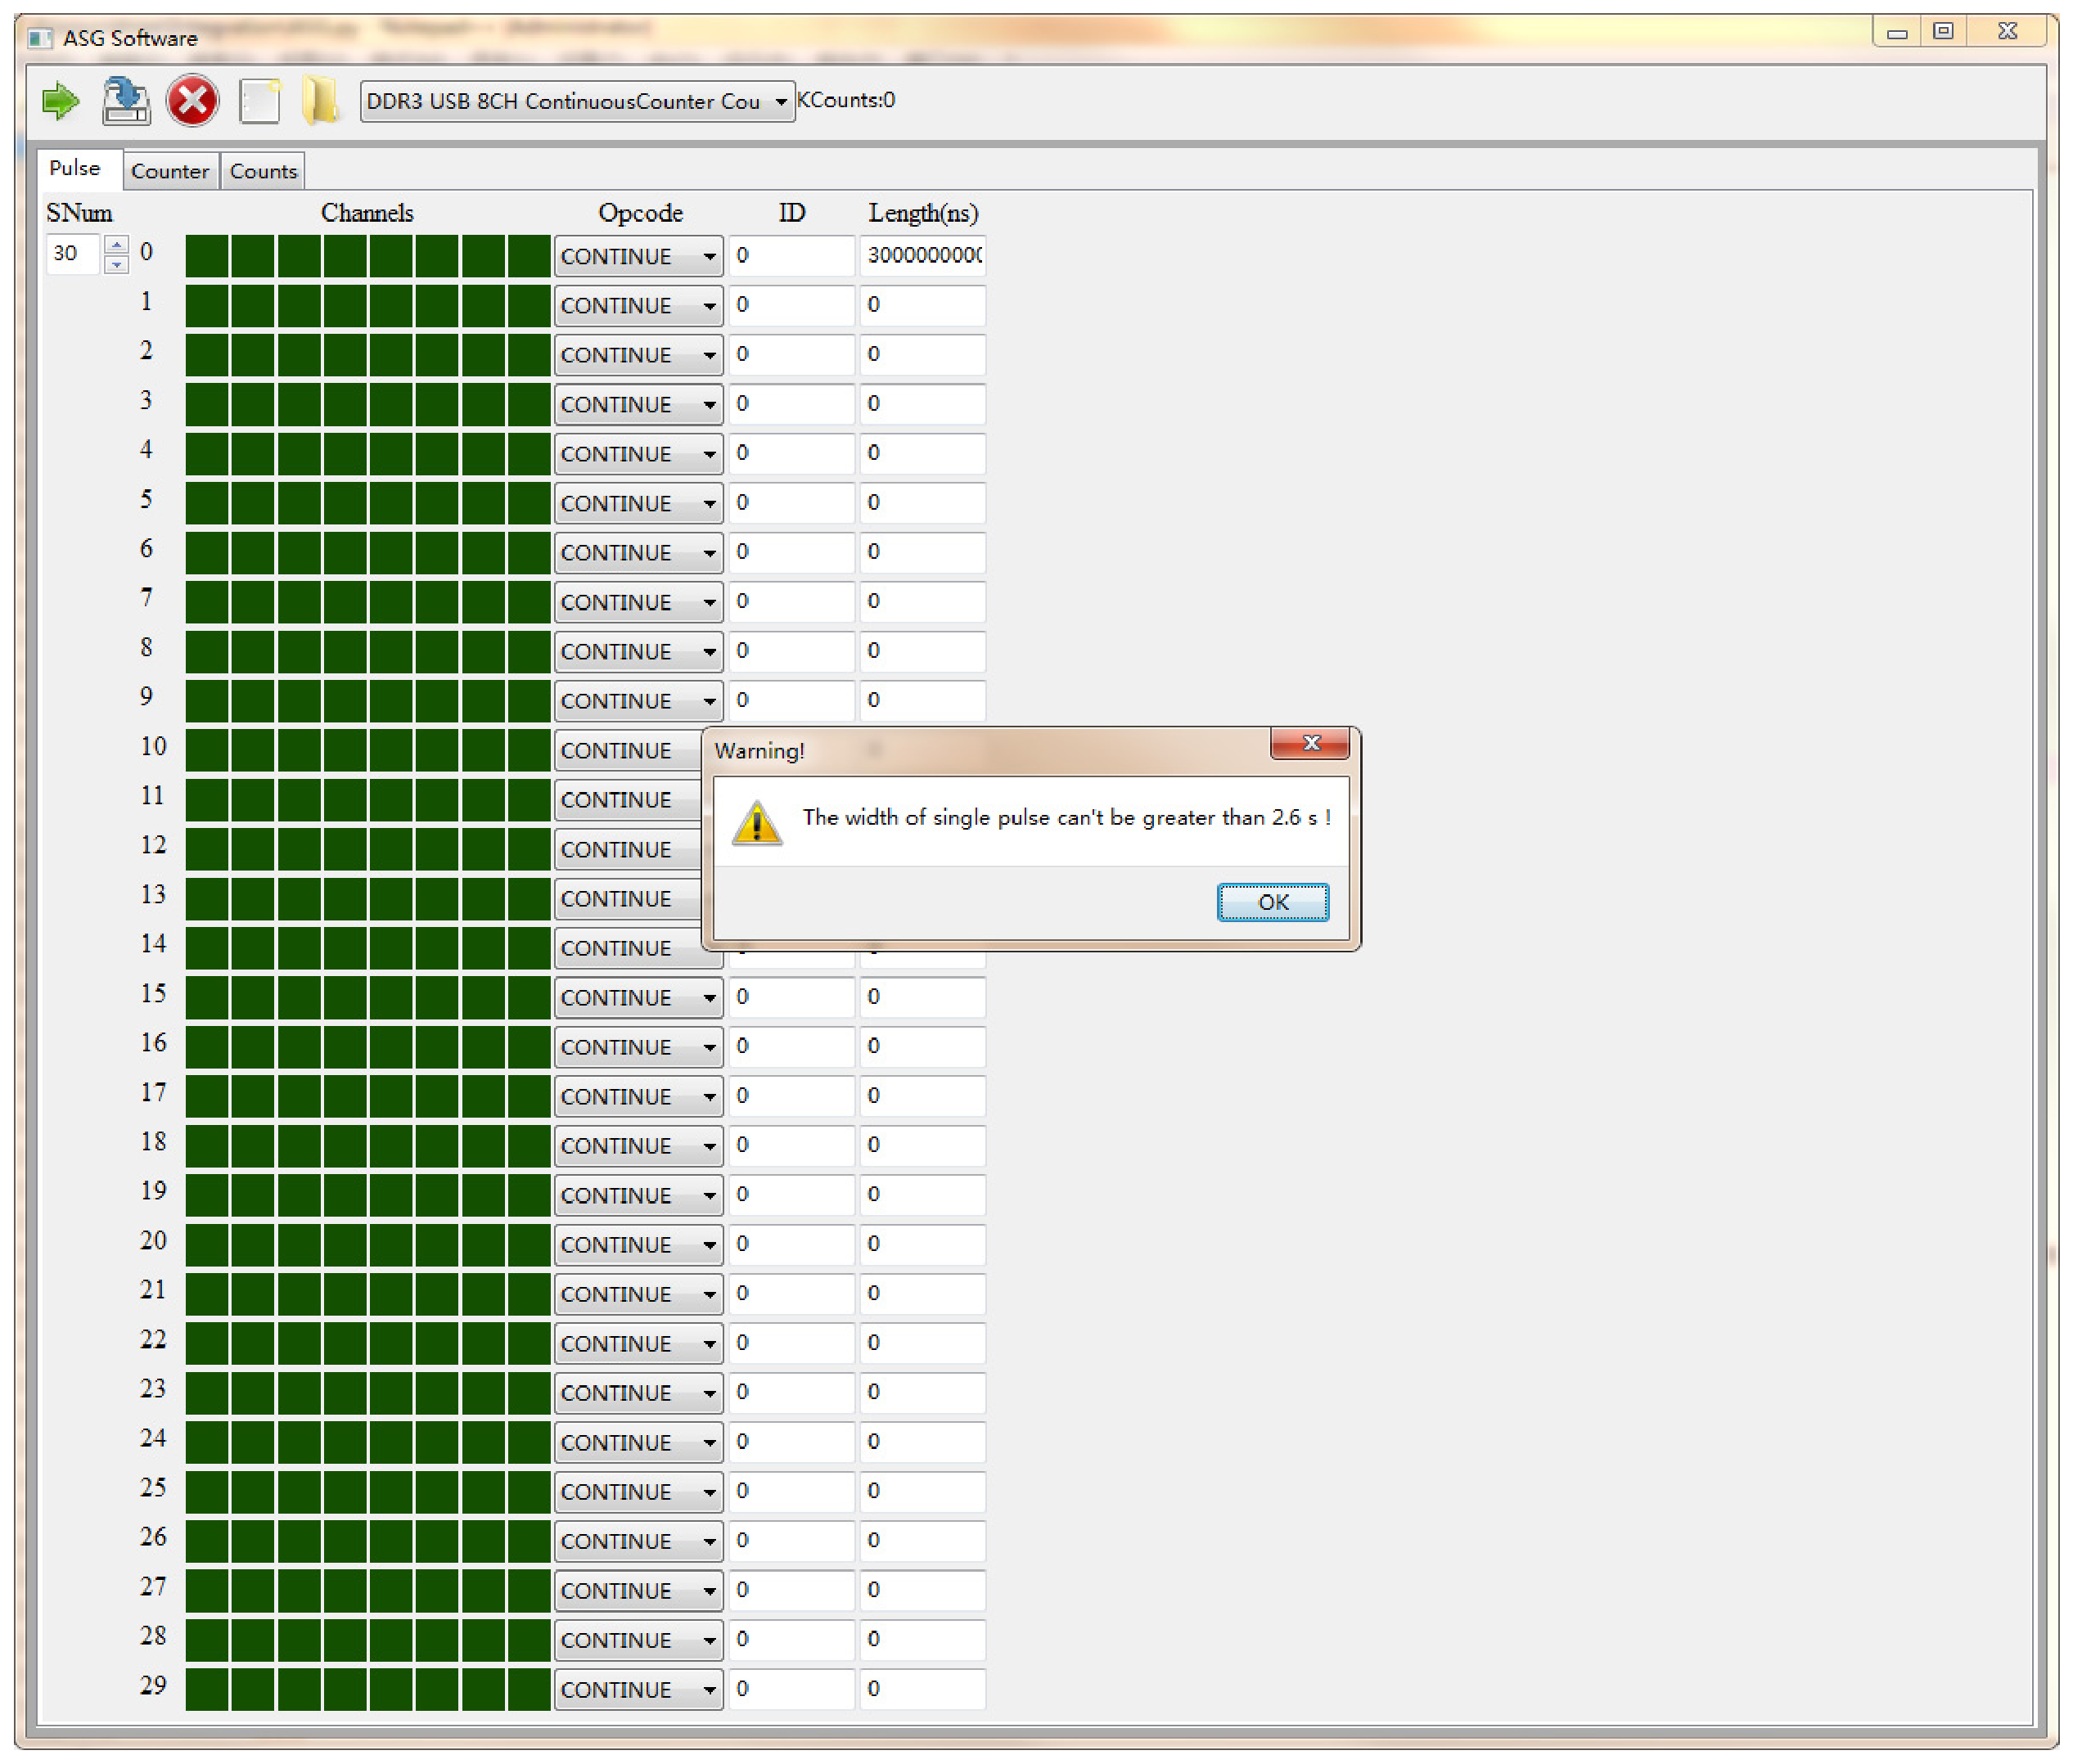
\includegraphics[width=11cm,height=9cm]{fig4_4}
%\includegraphics[height=9cm]{fig4_4yh}
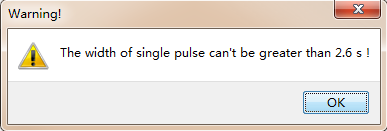
\includegraphics[height=3cm]{fig4_6_yh}
\caption{定义方波宽度大于2.6 s提示}
\end{figure}

\vspace{0.4cm}
\noindent \textbf{(3)}. 用户定义的每个方波序列的宽度必须是0.05 ns的整数倍。如图4.7,当用户定义的方波序列中存在单个方波脉冲宽度非0.05 ns整数倍时,软件会弹出提示对话框。

\vspace{0.2cm}
\begin{figure}[H]
\centering
%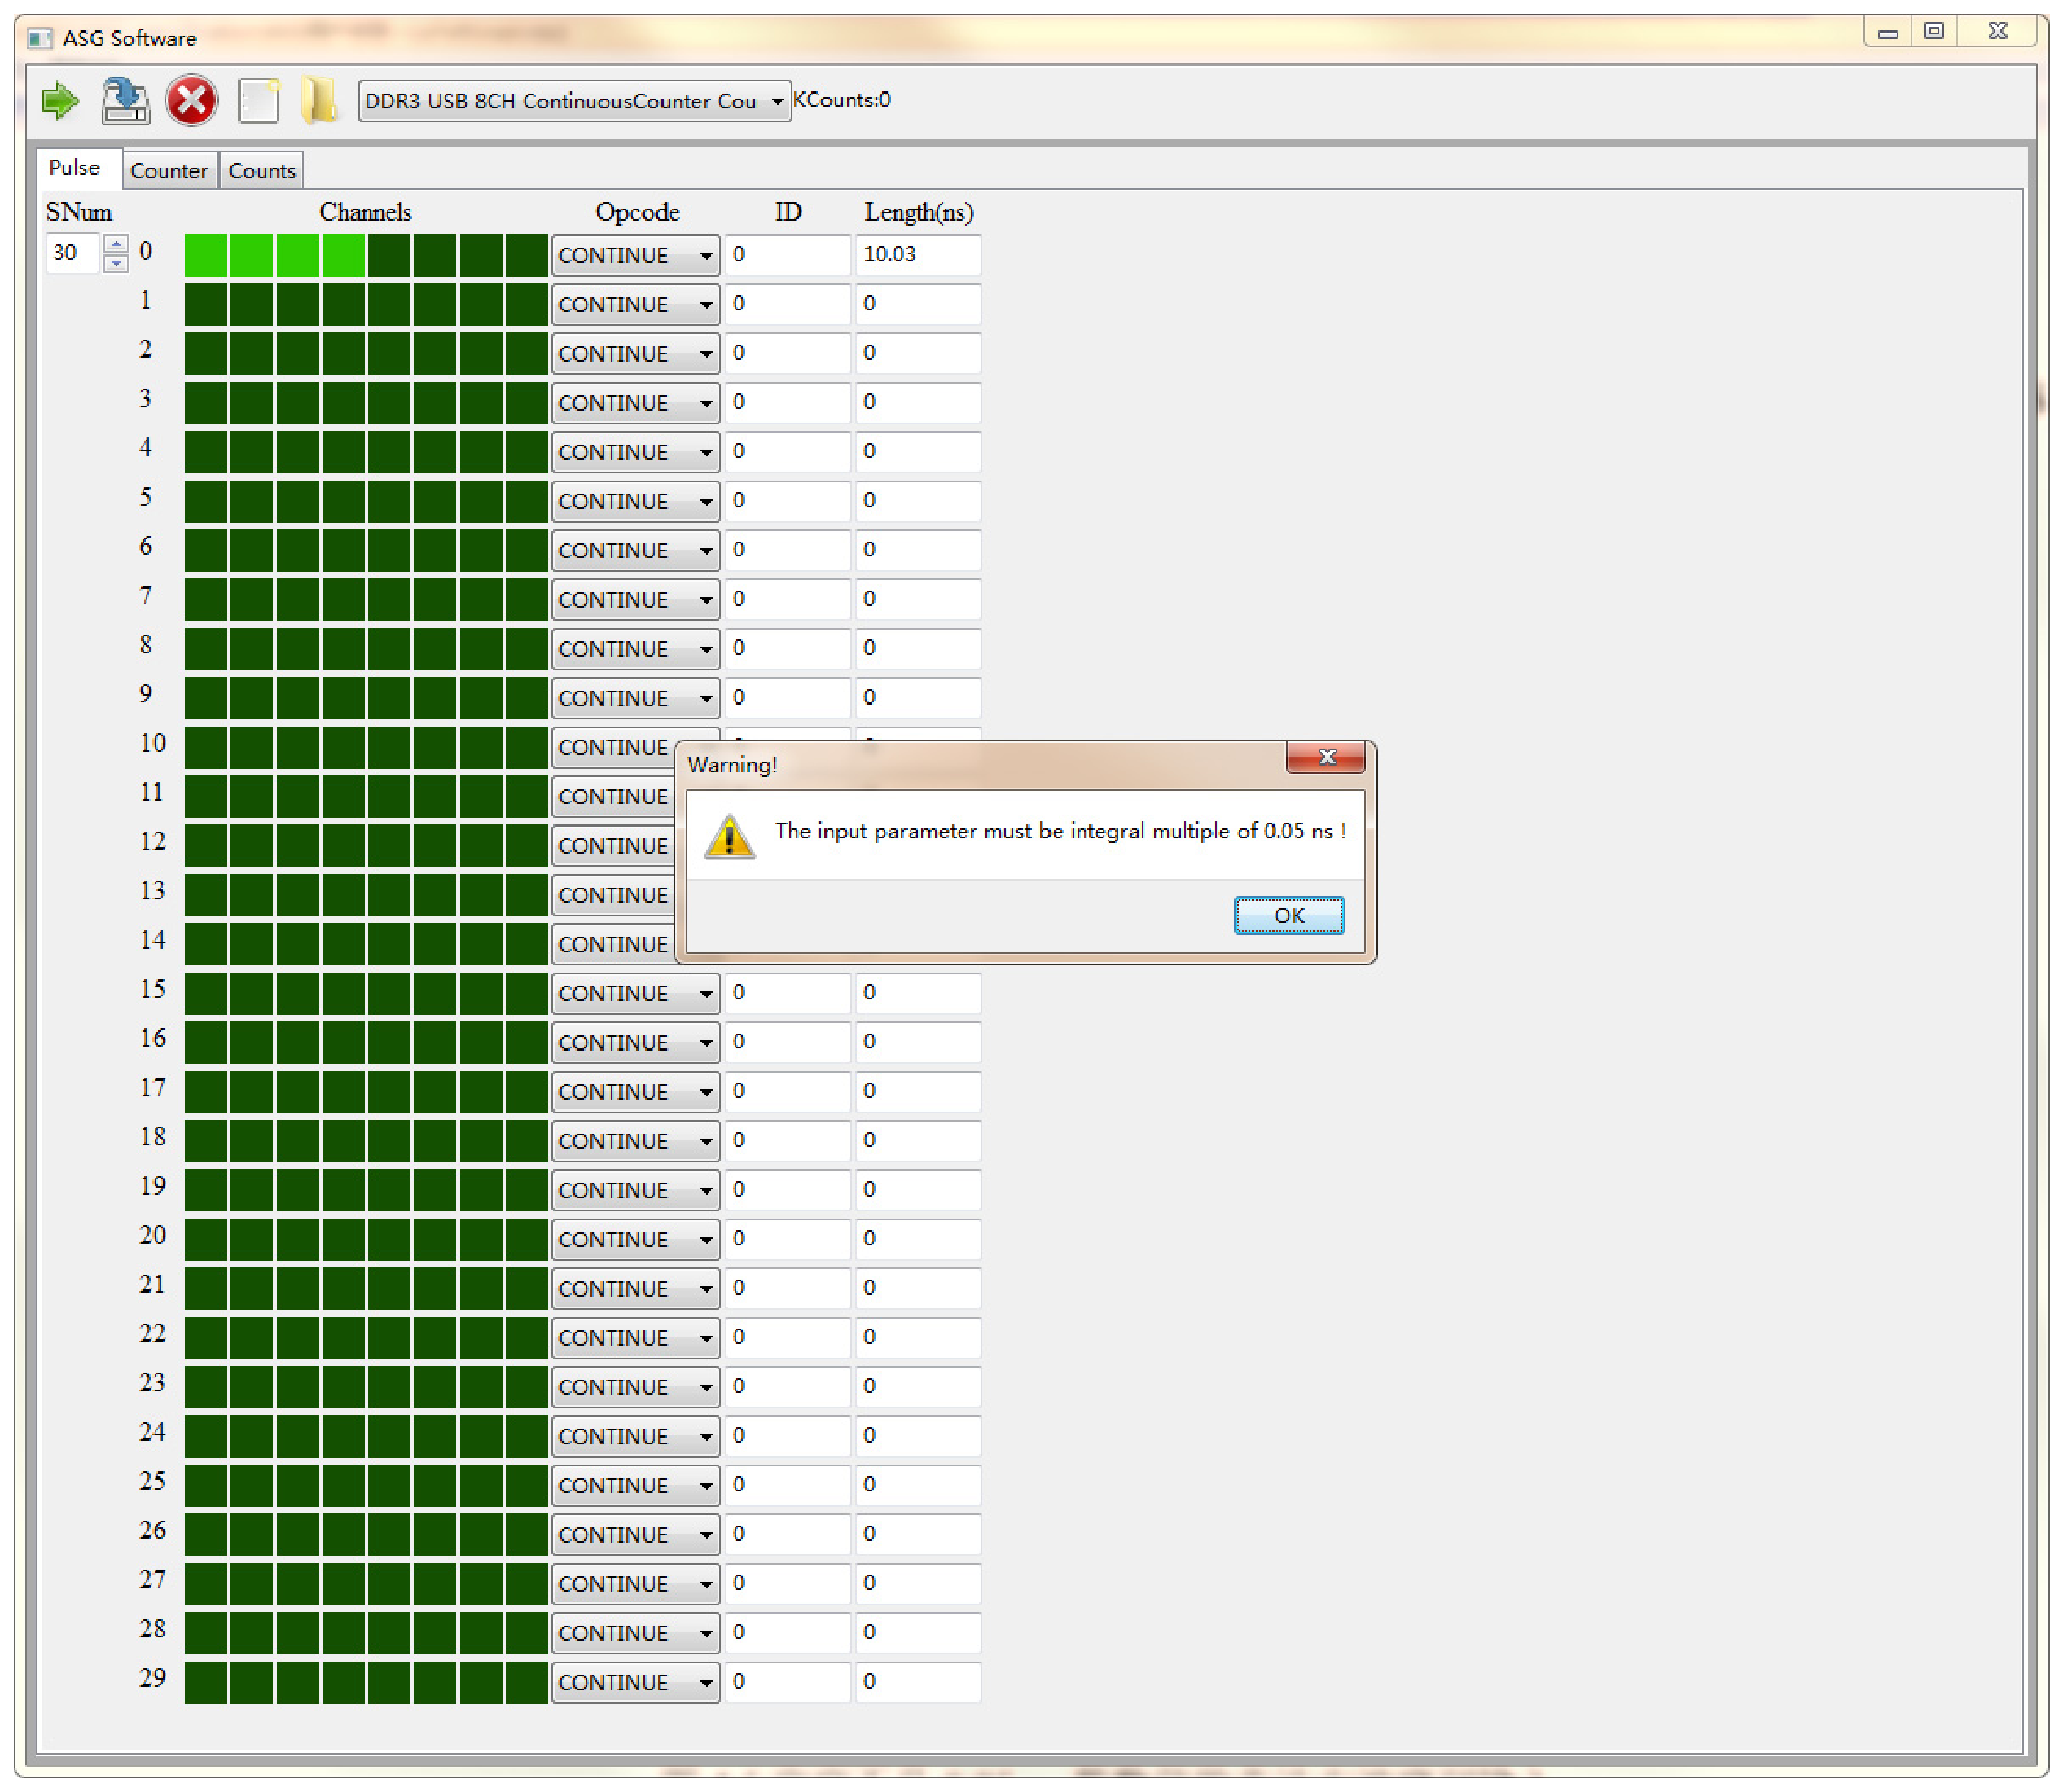
\includegraphics[width=11cm,height=9cm]{fig4_5}
%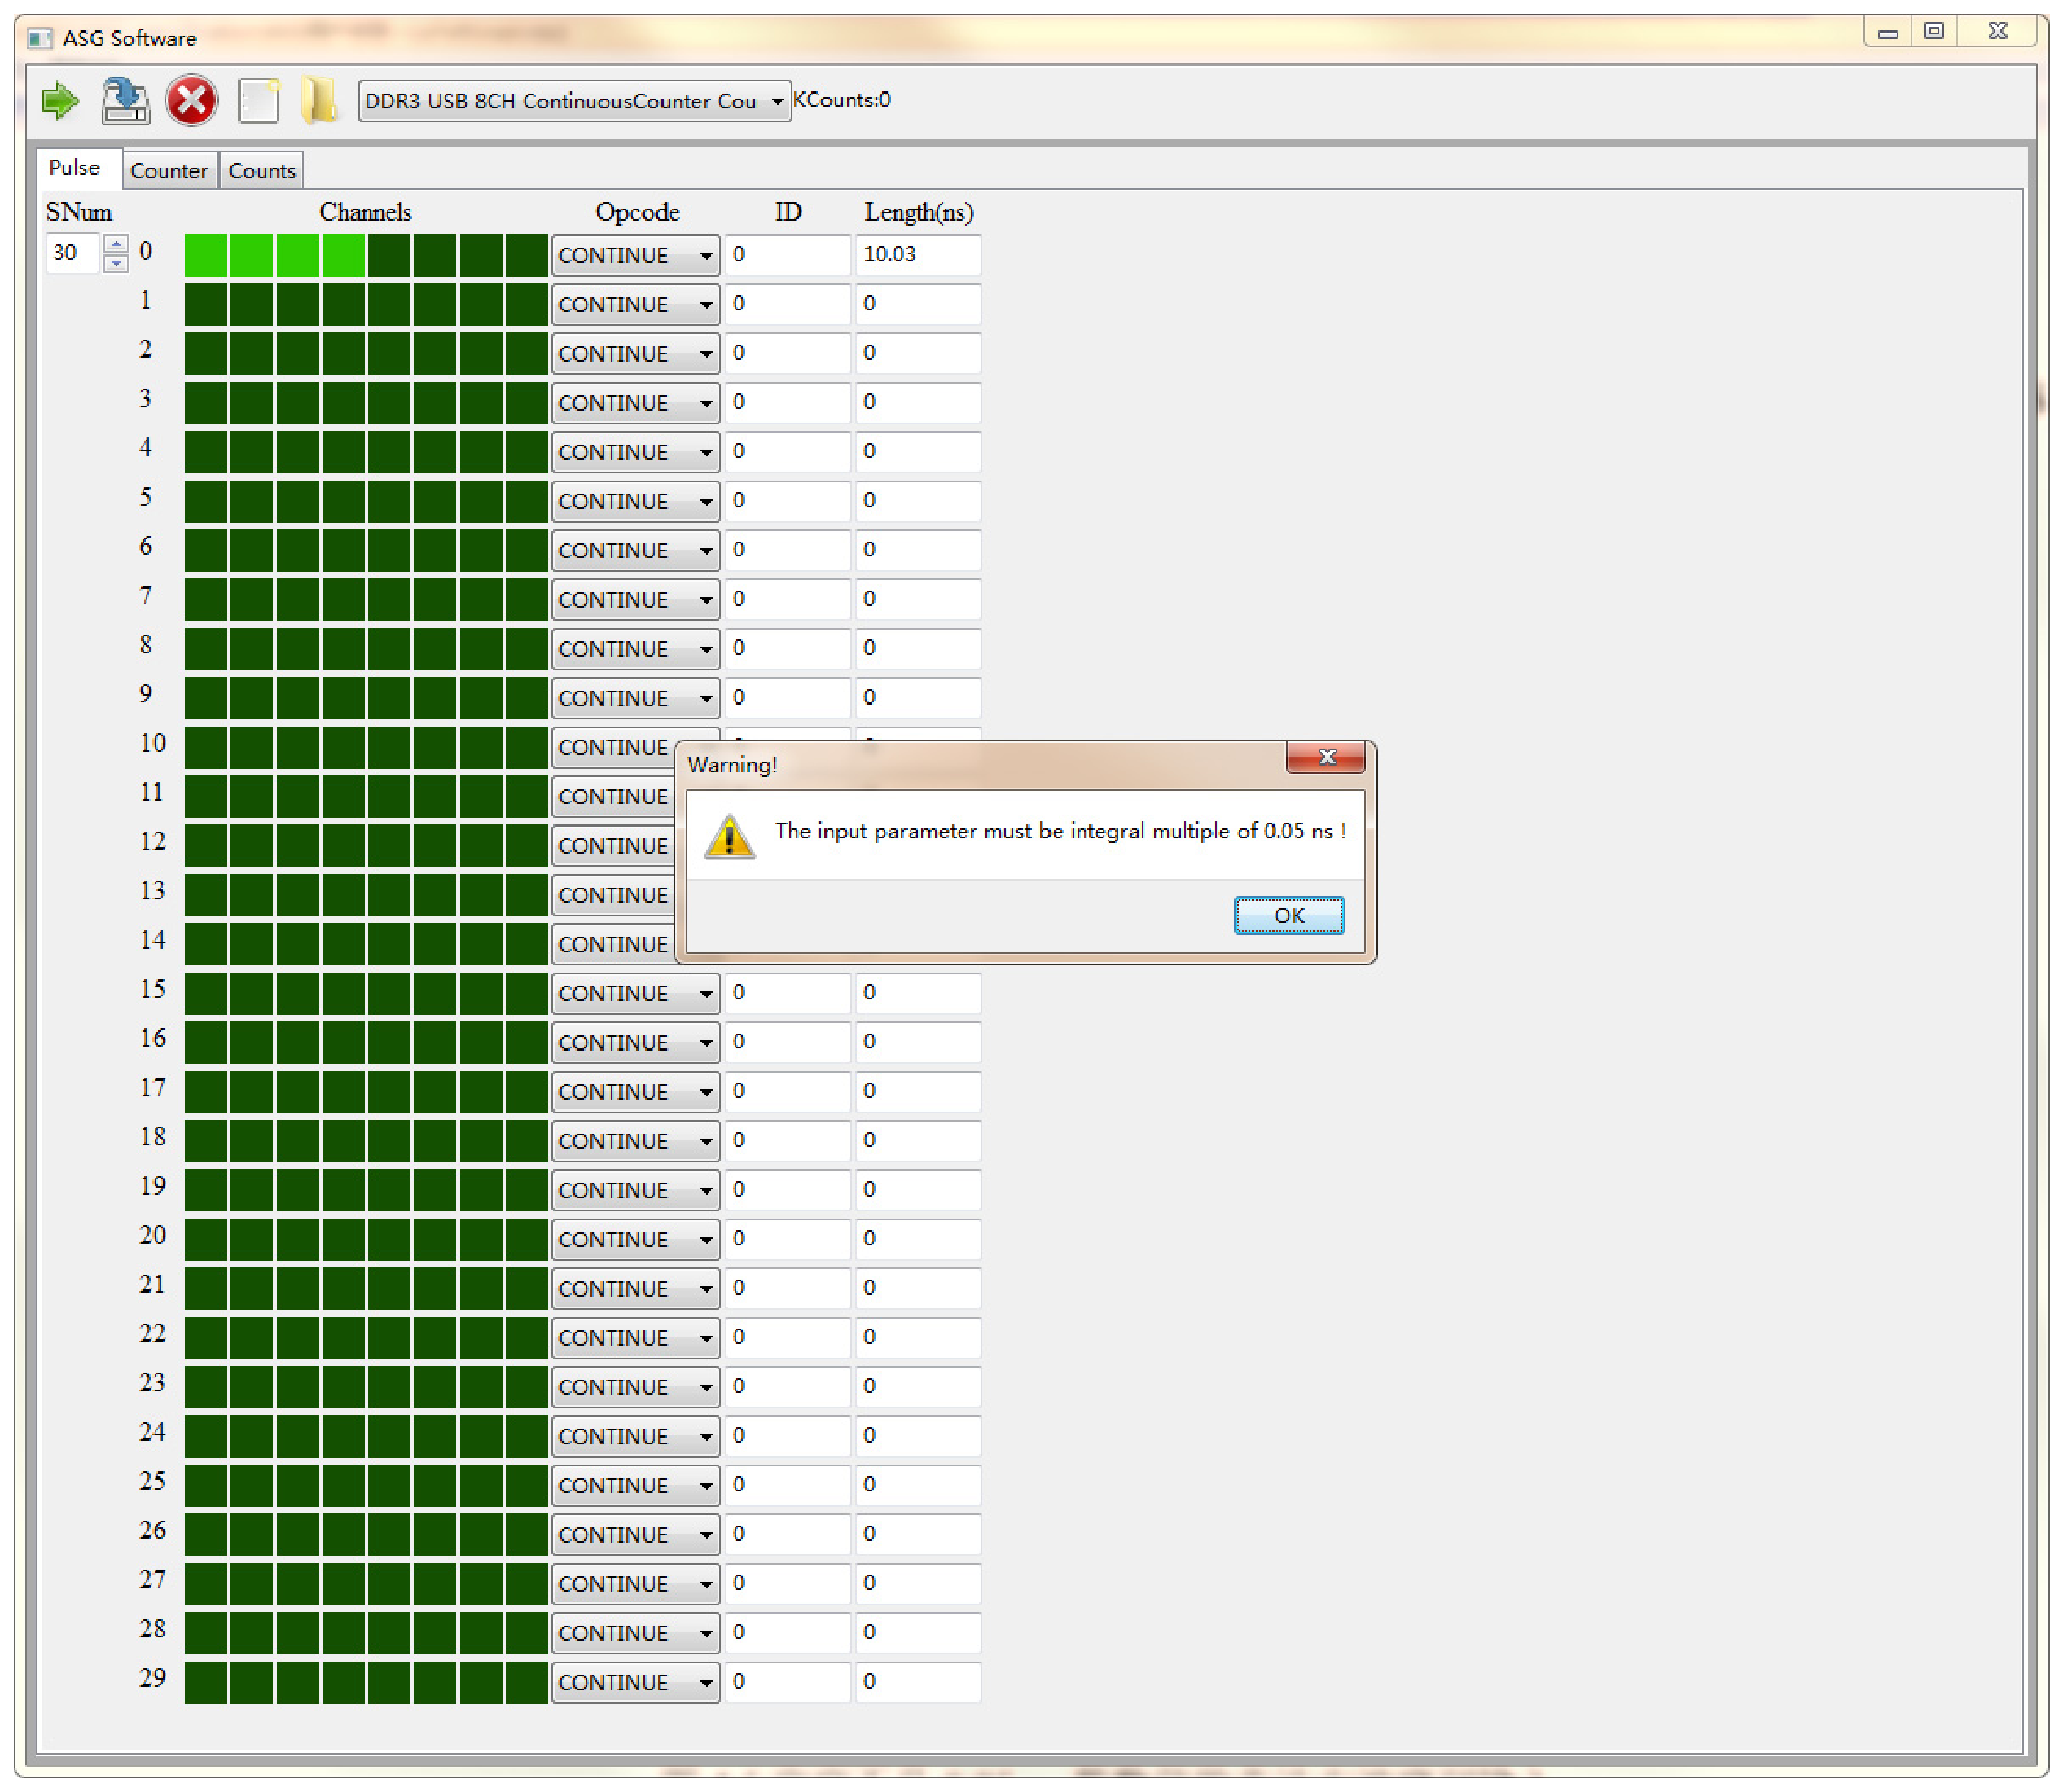
\includegraphics[height=9cm]{fig4_5}
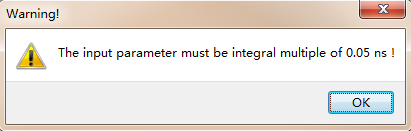
\includegraphics[height=3cm]{fig4_7_yh}
\caption{定义宽度不是0.05 ns整数倍提示}
\end{figure}

%\newpage
%\section{\heiti 开始播放方波序列}
%用户点击“Download”按钮
%
\includegraphics{download},可将自定义方波序列数据下载到硬件中。点击“Start”按钮{ }{ }
\includegraphics[height=0.7cm]{start},可使仪器各输出通道开始同步播放用户自定义的方波序列,在点击“Start” 按钮之前必须先将方波序列数据下载到硬件中。将输出通道用同轴线连接至示波器上可以看到仪器输出的方波波形。
%
%\section{\heiti 停止播放方波序列}
%当仪器正在播放方波序列时,可以通过点击“Stop”按钮{ }{ }
\includegraphics[height=0.7cm]{stop}使仪器停止播放方波序列。





